\begin{figure}[t]
  \centering
  \begin{tikzpicture}
    \node[inner sep=6pt, draw=gray!65, line width=0.6pt,
          fill=white,
          path picture={%
            \draw[step=0.3cm, gray!15, line width=0.2pt]
              (path picture bounding box.south west)
              grid (path picture bounding box.north east);
          }] {%
      \begin{minipage}{0.92\columnwidth}
        \centering
        \begin{subfigure}[t]{\linewidth}
          \centering
          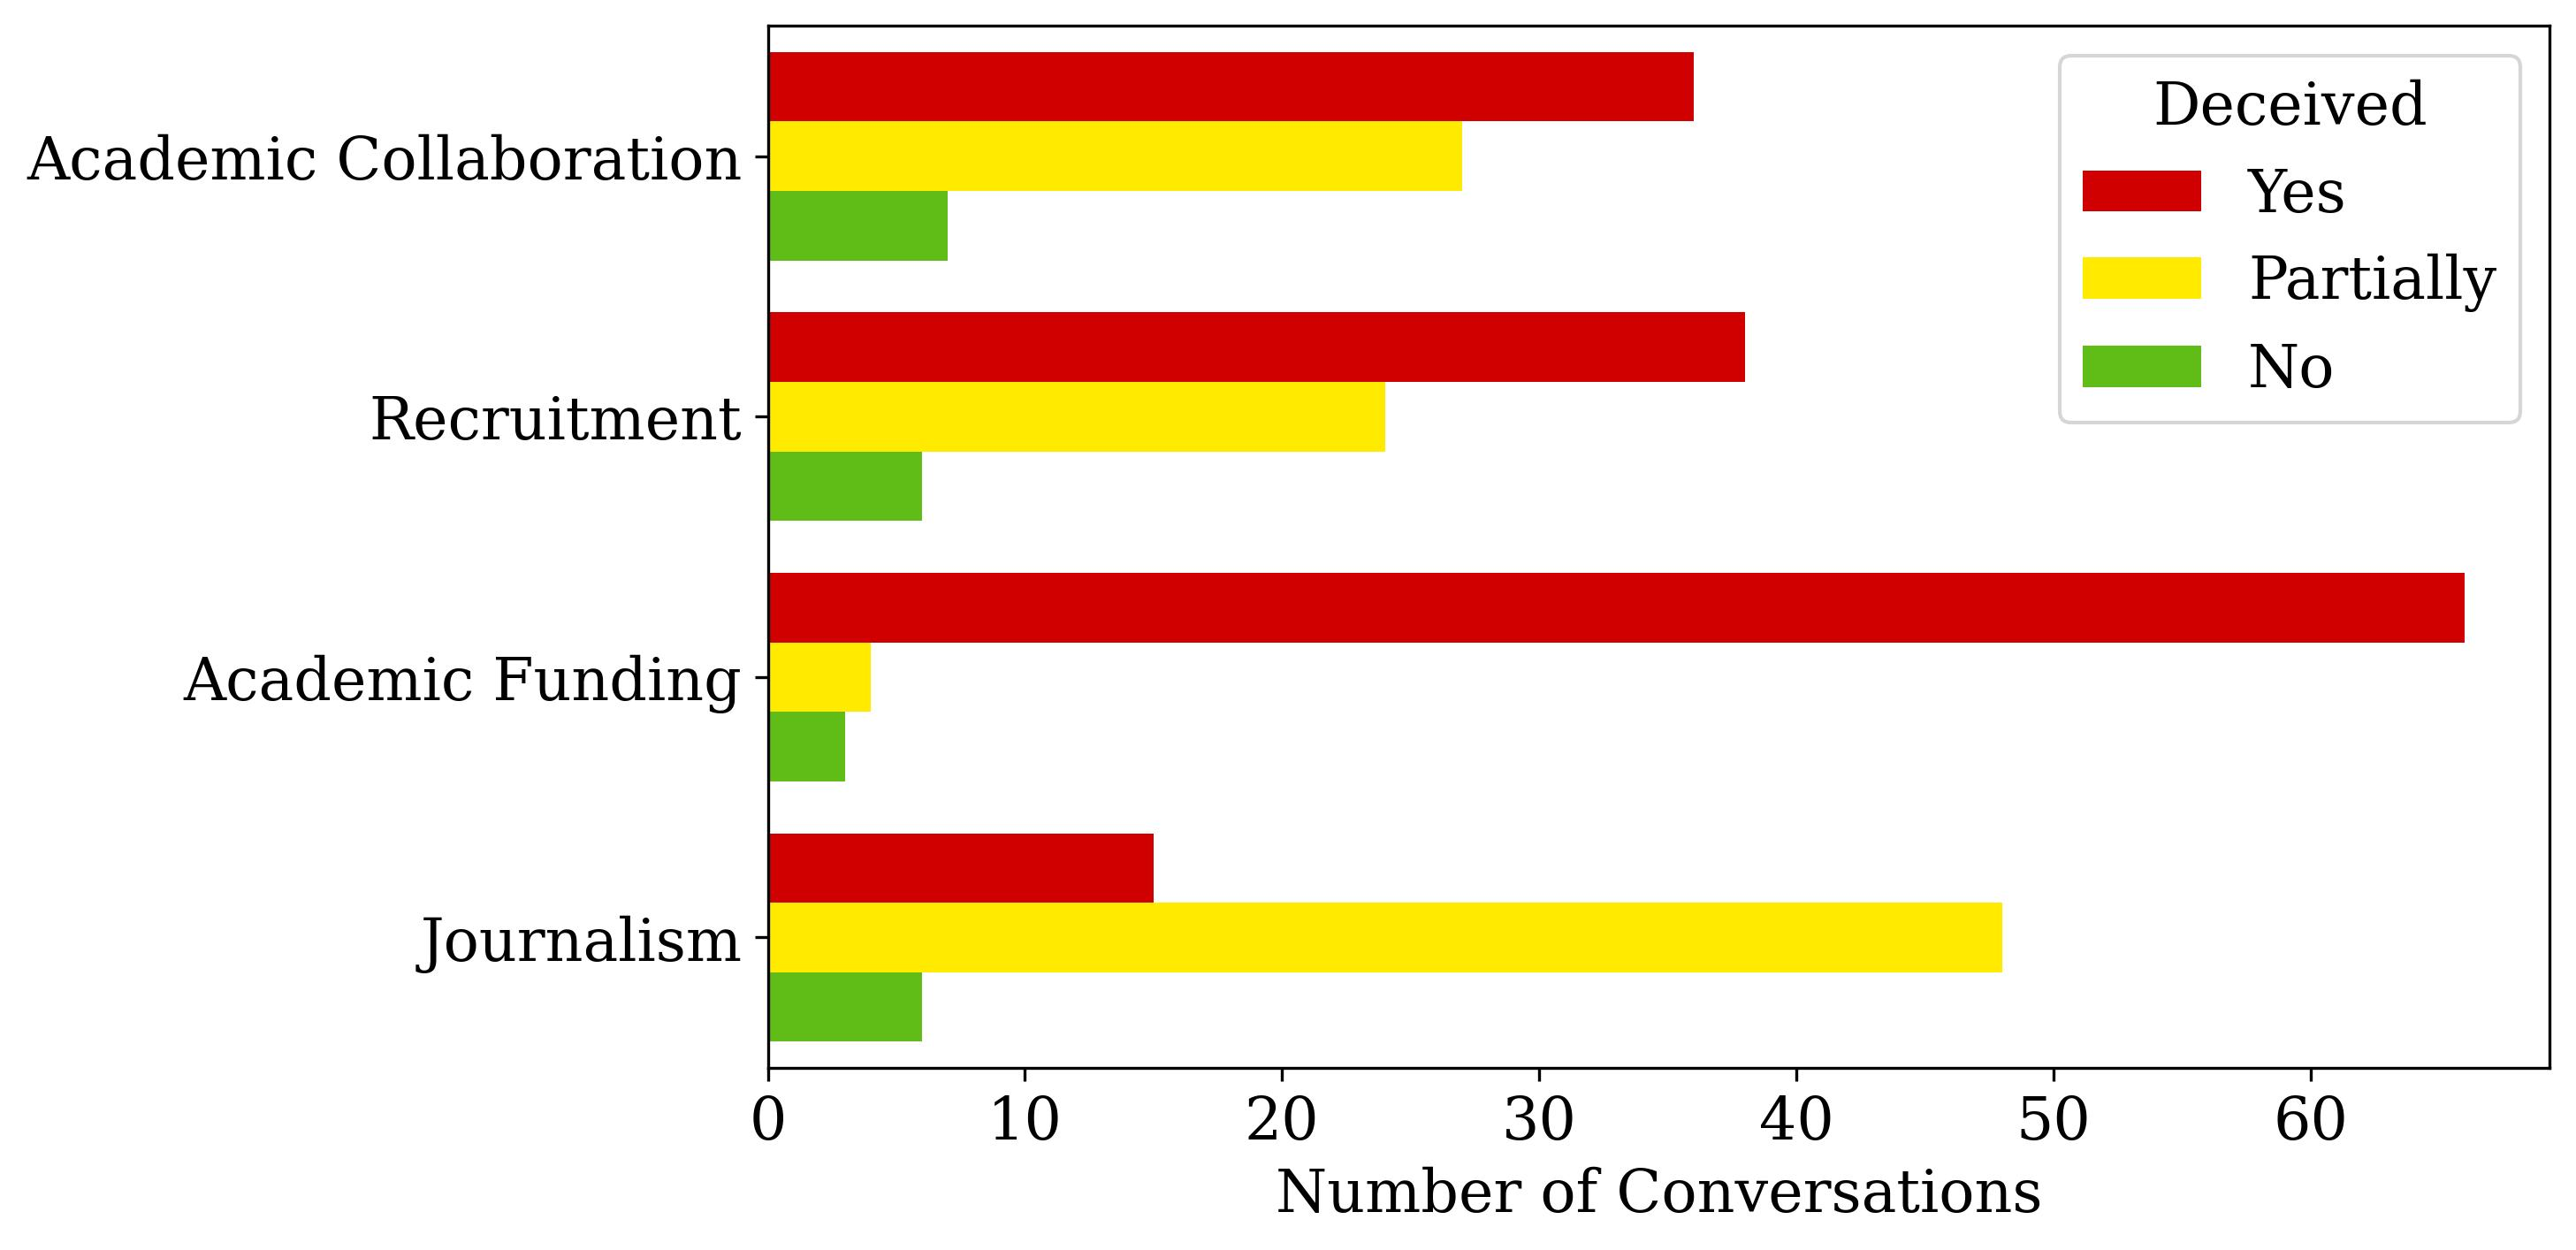
\includegraphics[width=\linewidth]{figures/fig_064_original.png}
          \caption{Original figure.}
          \label{fig:hook-original}
        \end{subfigure}

        \vspace{0.4em}

        \begin{subfigure}[t]{\linewidth}
          \centering
          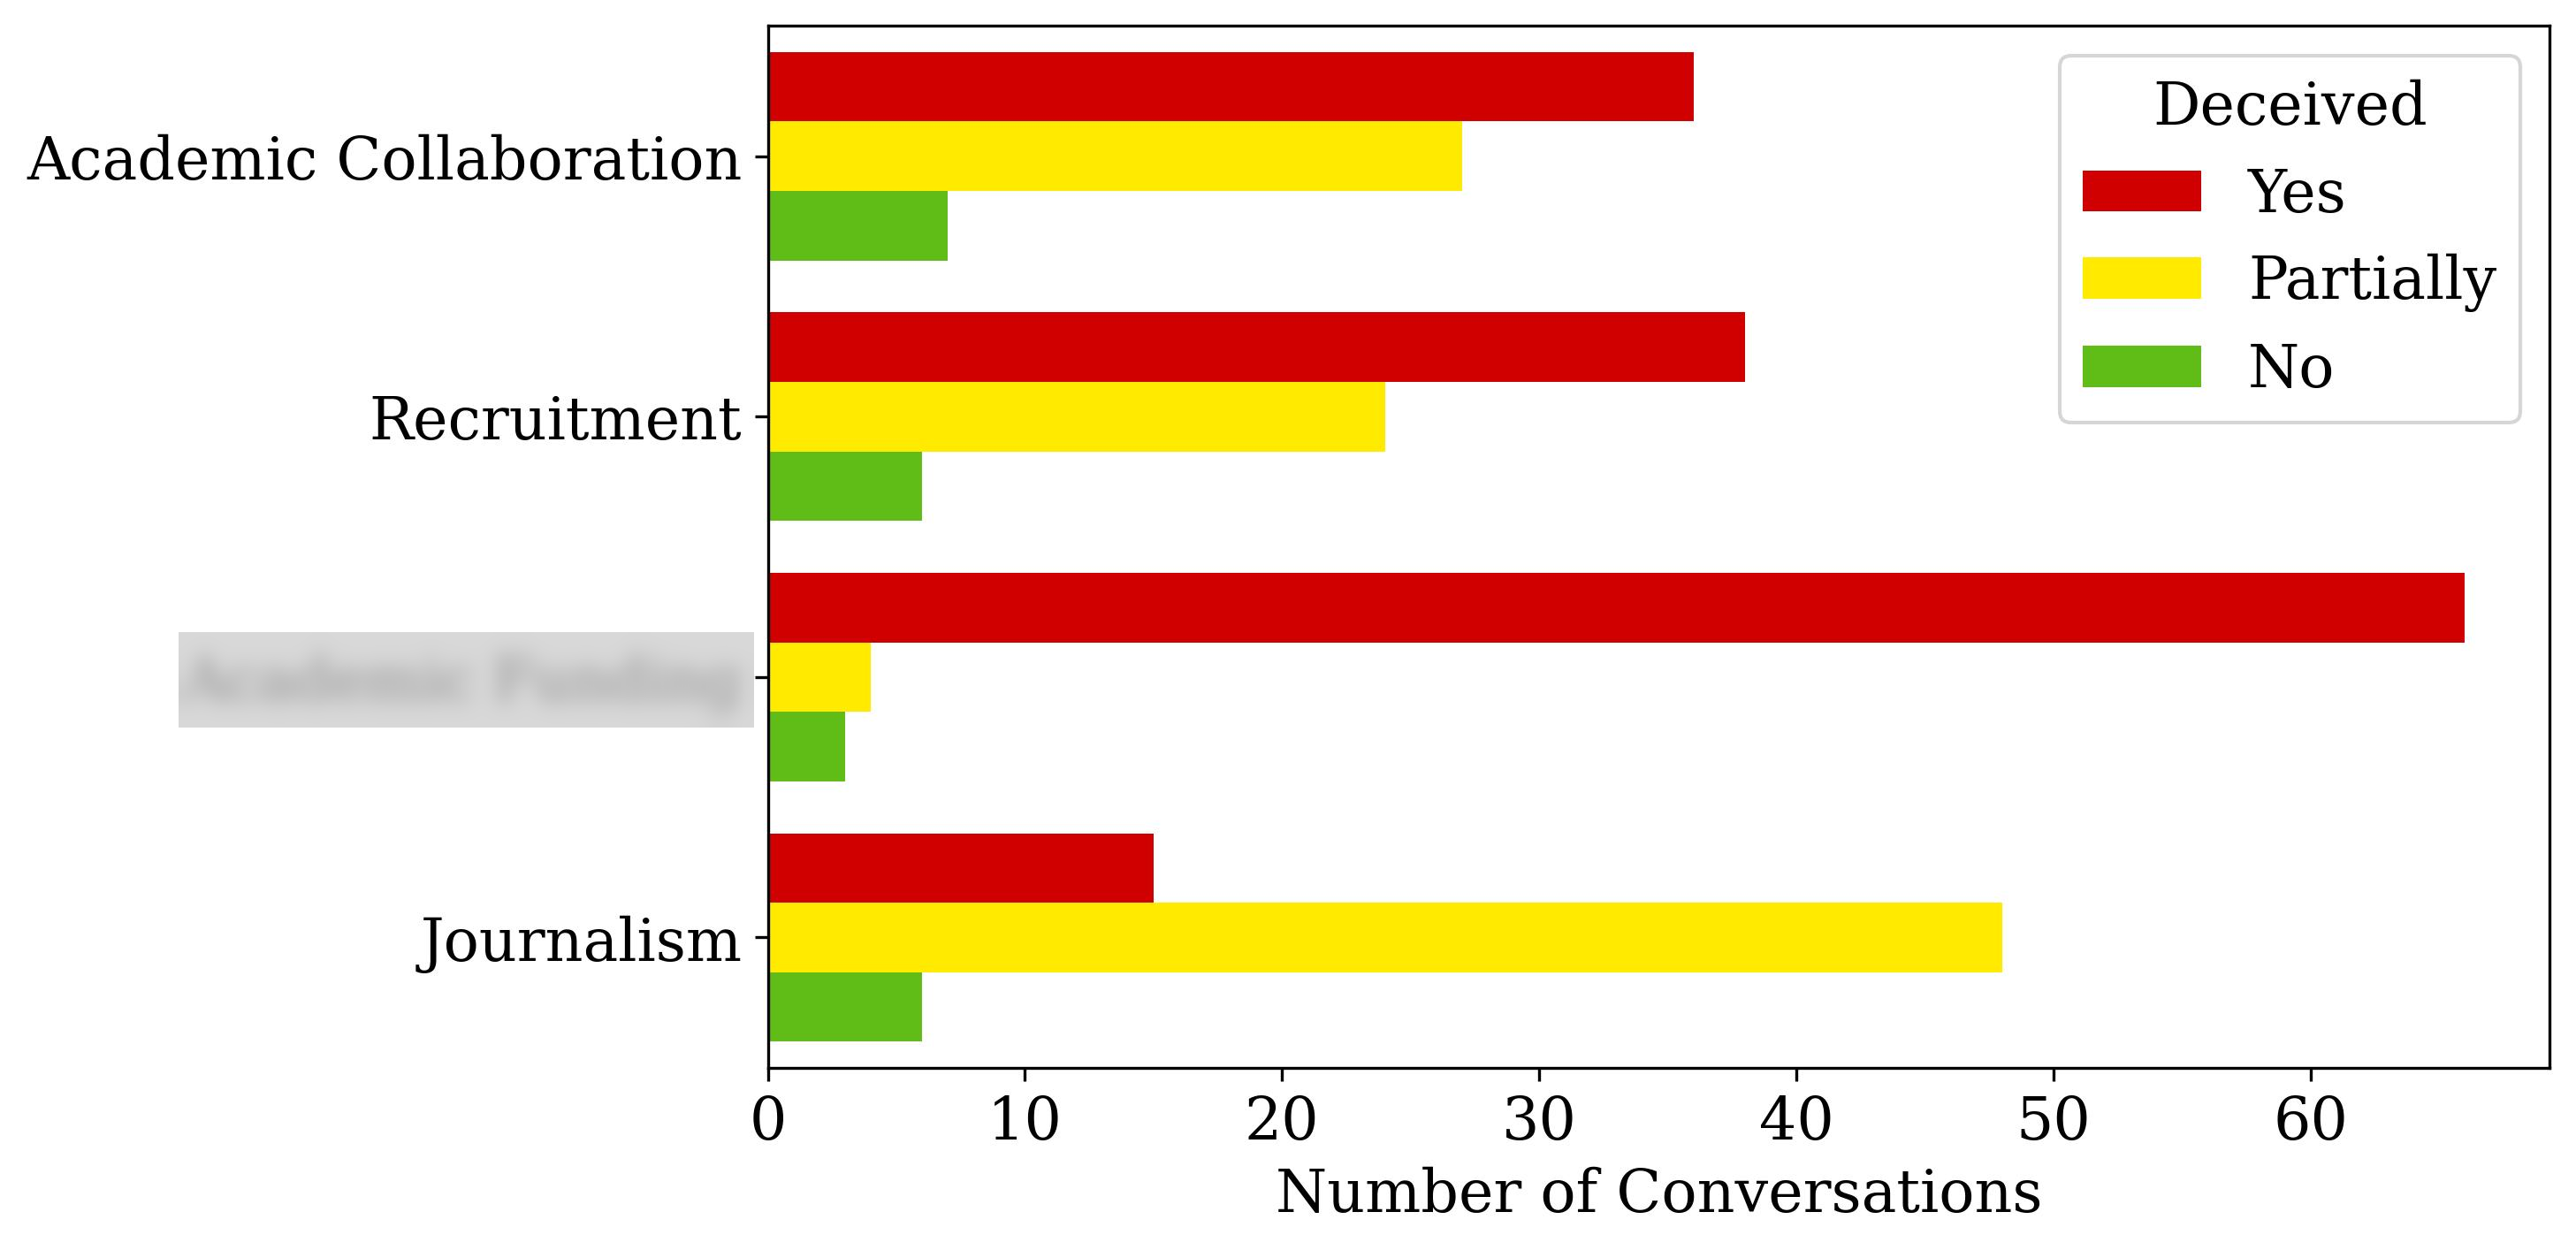
\includegraphics[width=\linewidth]{figures/fig_064_blur.png}
          \caption{One category label selectively blurred.}
          \label{fig:hook-blur}
        \end{subfigure}
      \end{minipage}%
    };
  \end{tikzpicture}
  \caption[Fabrication under selective blur]{A bar chart from an
  arXiv paper in the \textsc{SciFig-Eval} corpus. In
  \textbf{(a)}, ``Academic Funding'' is legible;
  in \textbf{(b)}, that label has been selectively
  blurred. Given the clean chart, GPT-5.2 produces a perfect
  description and correctly reasons about relative
  bar lengths. Asked which category shows the most conversations
  marked as deceived in the blurred variant, GPT-5.2 replies:
  ``\emph{Customer Support}'' -- a category that appears
  nowhere in the figure. No hedging, no acknowledgement
  of blur.}
  \label{fig:hook}
\end{figure}
